\documentclass[12pt]{article}
\usepackage{amsmath}
\usepackage{setspace}
\usepackage{adjustbox}
\usepackage{graphicx}
\usepackage{float}
\usepackage{multicol}
\usepackage{hyperref}
\usepackage{subfig}
\usepackage{wrapfig}
\usepackage{xcolor}
\usepackage{tabularray}
\usepackage{sidecap}
%\usepackage{natbib,url}
\usepackage[backend=biber,style=numeric,maxnames =2,giveninits = true]{biblatex}
\addbibresource{journal_abbreviations.bib}
\addbibresource{References.bib}
\usepackage[margin = 1in]{geometry}
\usepackage{fancyhdr}
\usepackage{sectsty}
\usepackage{titlesec}


\sectionfont{\fontsize{14}{15}\selectfont}
\subsectionfont{\fontsize{12}{15}\selectfont}
%\bibliographystyle{abbrv}
\DeclareBibliographyDriver{std}{%
  \usebibmacro{bibindex}%
  \usebibmacro{begentry}%
  \usebibmacro{author/editor+others/translator+others}%
  \usebibmacro{title}%
  \setunit{\labelnamepunct}\newblock
  %\usebibmacro{title}%
    %\newunit\newblock
  \usebibmacro{journal}
  \newunit\newblock
  \usebibmacro{date}%
  \newunit\newblock
\usebibmacro{finentry}}

\DeclareBibliographyDriver{stdbook}{%
  \usebibmacro{bibindex}%
  \usebibmacro{begentry}%
  \usebibmacro{author/editor+others/translator+others}%
  \setunit{\labelnamepunct}\newblock
  %\usebibmacro{title}%
  \usebibmacro{title}
  \newunit\newblock
  \usebibmacro{date}%
  \newunit\newblock
\usebibmacro{finentry}}

%\DeclareBibliographyAlias{article}{std}
%\DeclareBibliographyAlias{book}{stdbook}
%\DeclareBibliographyAlias{misc}{stdbook}
\AtEveryBibitem{% Clean up the bibtex rather than editing it
 \clearfield{isbn}
 \clearfield{doi}
 \clearfield{issn}
 }
\AtBeginBibliography{\small}
\definecolor{gray_c}{rgb}{0.745, 0.898, 0.898}
\definecolor{gray_h}{rgb}{0.43, 0.72, 0.72}

%\titlespacing\section{0pt}{12pt plus 4pt minus 2pt}{0pt plus 2pt minus 2pt}
\titlespacing\subsection{0pt}{12pt plus 4pt minus 2pt}{0pt plus 2pt minus 2pt}
%\titlespacing\subsubsection{0pt}{12pt plus 4pt minus 2pt}{0pt plus 2pt minus 2pt}

\def\epo{\epsilon\rightarrow 0}
\def\lb{\left(}
\def\rb{\right)}
\def\ls{\left[ \vphantom]}
\def\rs{\right] }
\def\ep{\epsilon}

\title{Direct simulation of ocean-ice coupling in icy moons}
\author{Tobias Oliver}
\date{}

\begin{document}
\pagestyle{fancy}
\thispagestyle{fancy}
%... then configure it.
\fancyhf{} % clear all header fields
\fancyhead[L]{\textcolor{red}{Tobias Oliver\\
Research Proposal}}
\fancyfoot[R]{\thepage}
\newcommand{\citep}[1]{\cite{#1}}
\begin{center}
\large{\textbf{Dynamic ocean-ice coupling on icy moons}}
\end{center}

I propose to study the effects of salinity on convective processes in the icy moons of our Solar System and beyond. 
I will investigate the interplay of horizontal and bottom driven convection, and the competing effects of temperature and salinity via a novel suite of tailored numerical simulations. 
I will focus on the interaction between the subsurface oceans and the overlaying ice in order to understand their coupled dynamics. 
%\textbf{With upcoming data from the \textit{Europa Clipper} and \textit{JUICE} missions, the results from this study can be used to relate surface observations to ocean dynamics}.
\textbf{The proposed work is relevant to a broad range of planetary bodies, including icy moons and exoplanets.} A specific application is to serve the \textit{Europa Clipper} and \textit{JUICE} space missions by providing insight for relating upcoming data to underlying ocean dynamics and its coupling with the ice crust.

\section{Background}
Planetary bodies with liquid oceans are often considered to be suitable candidates for the habitability of life \citep{tB24}.
The Jovian satellites Europa, Callisto, and Ganymede, as well as the Saturnian moon Enceladus, were all identified as likely ocean worlds after data returned from the \textit{Galileo} and \textit{Cassini} missions \citep{fN16}. It has been suggested that a large portion of identified exoplanets contain subsurface oceans as well\citep{lQ20}.
Figure \ref{f:pic}(a) illustrates a proposed structure of these bodies. 

The sub-surface oceans link the solid cores of these planets and moons to their icy exteriors. Circulations within the oceans govern the transport of heat and chemicals to the icy surface \citep{kS20}. 

%It is likely that these oceans are turbulent and capable of convecting heat and chemicals between the solid interior and icy crust
%.
%A variety of forcing mechanisms have been proposed and discussed, such as electromagnetic coupling\citep{cGlP19}, tides, and precession\citep{kS24}, and in this investigation 
These oceans are believed to be extremely turbulent, and multiple mechanisms for driving circulation have been proposed \citep{kS24}.
%Multiple mechanisms are proposed to drive circulations in these ocean, which are believed to be extremely turbulent \cite{kS24}.
%The circulations in these oceans are driven by multiple mechanisms, and are believed to be extremely turbulent \citep{kS24}.
I propose to study buoyancy driven flows, in which variations in the fluid density drive convection.
I will consider the contributions of temperature and salinity to density variations.
%ensity variations are due to heterogeneities in both temperature and salinity.
%Heterogeneities in both temperature and salinity contribute to density variations.
%Density variations are usually attributed to two separate mechanisms-- heterogeneities in temperature and salinity. The associate density variations drives convection and references \citep{yA21,wK22} predict that this mechanism serves to flatten the ice shell of Europa (ie.  homogenous thickness).

%\begin{wrapfigure}{R}{0.6\textwidth}
%\end{wrapfigure}
\begin{figure}[H]
	\begin{center}
		\subfloat[][]{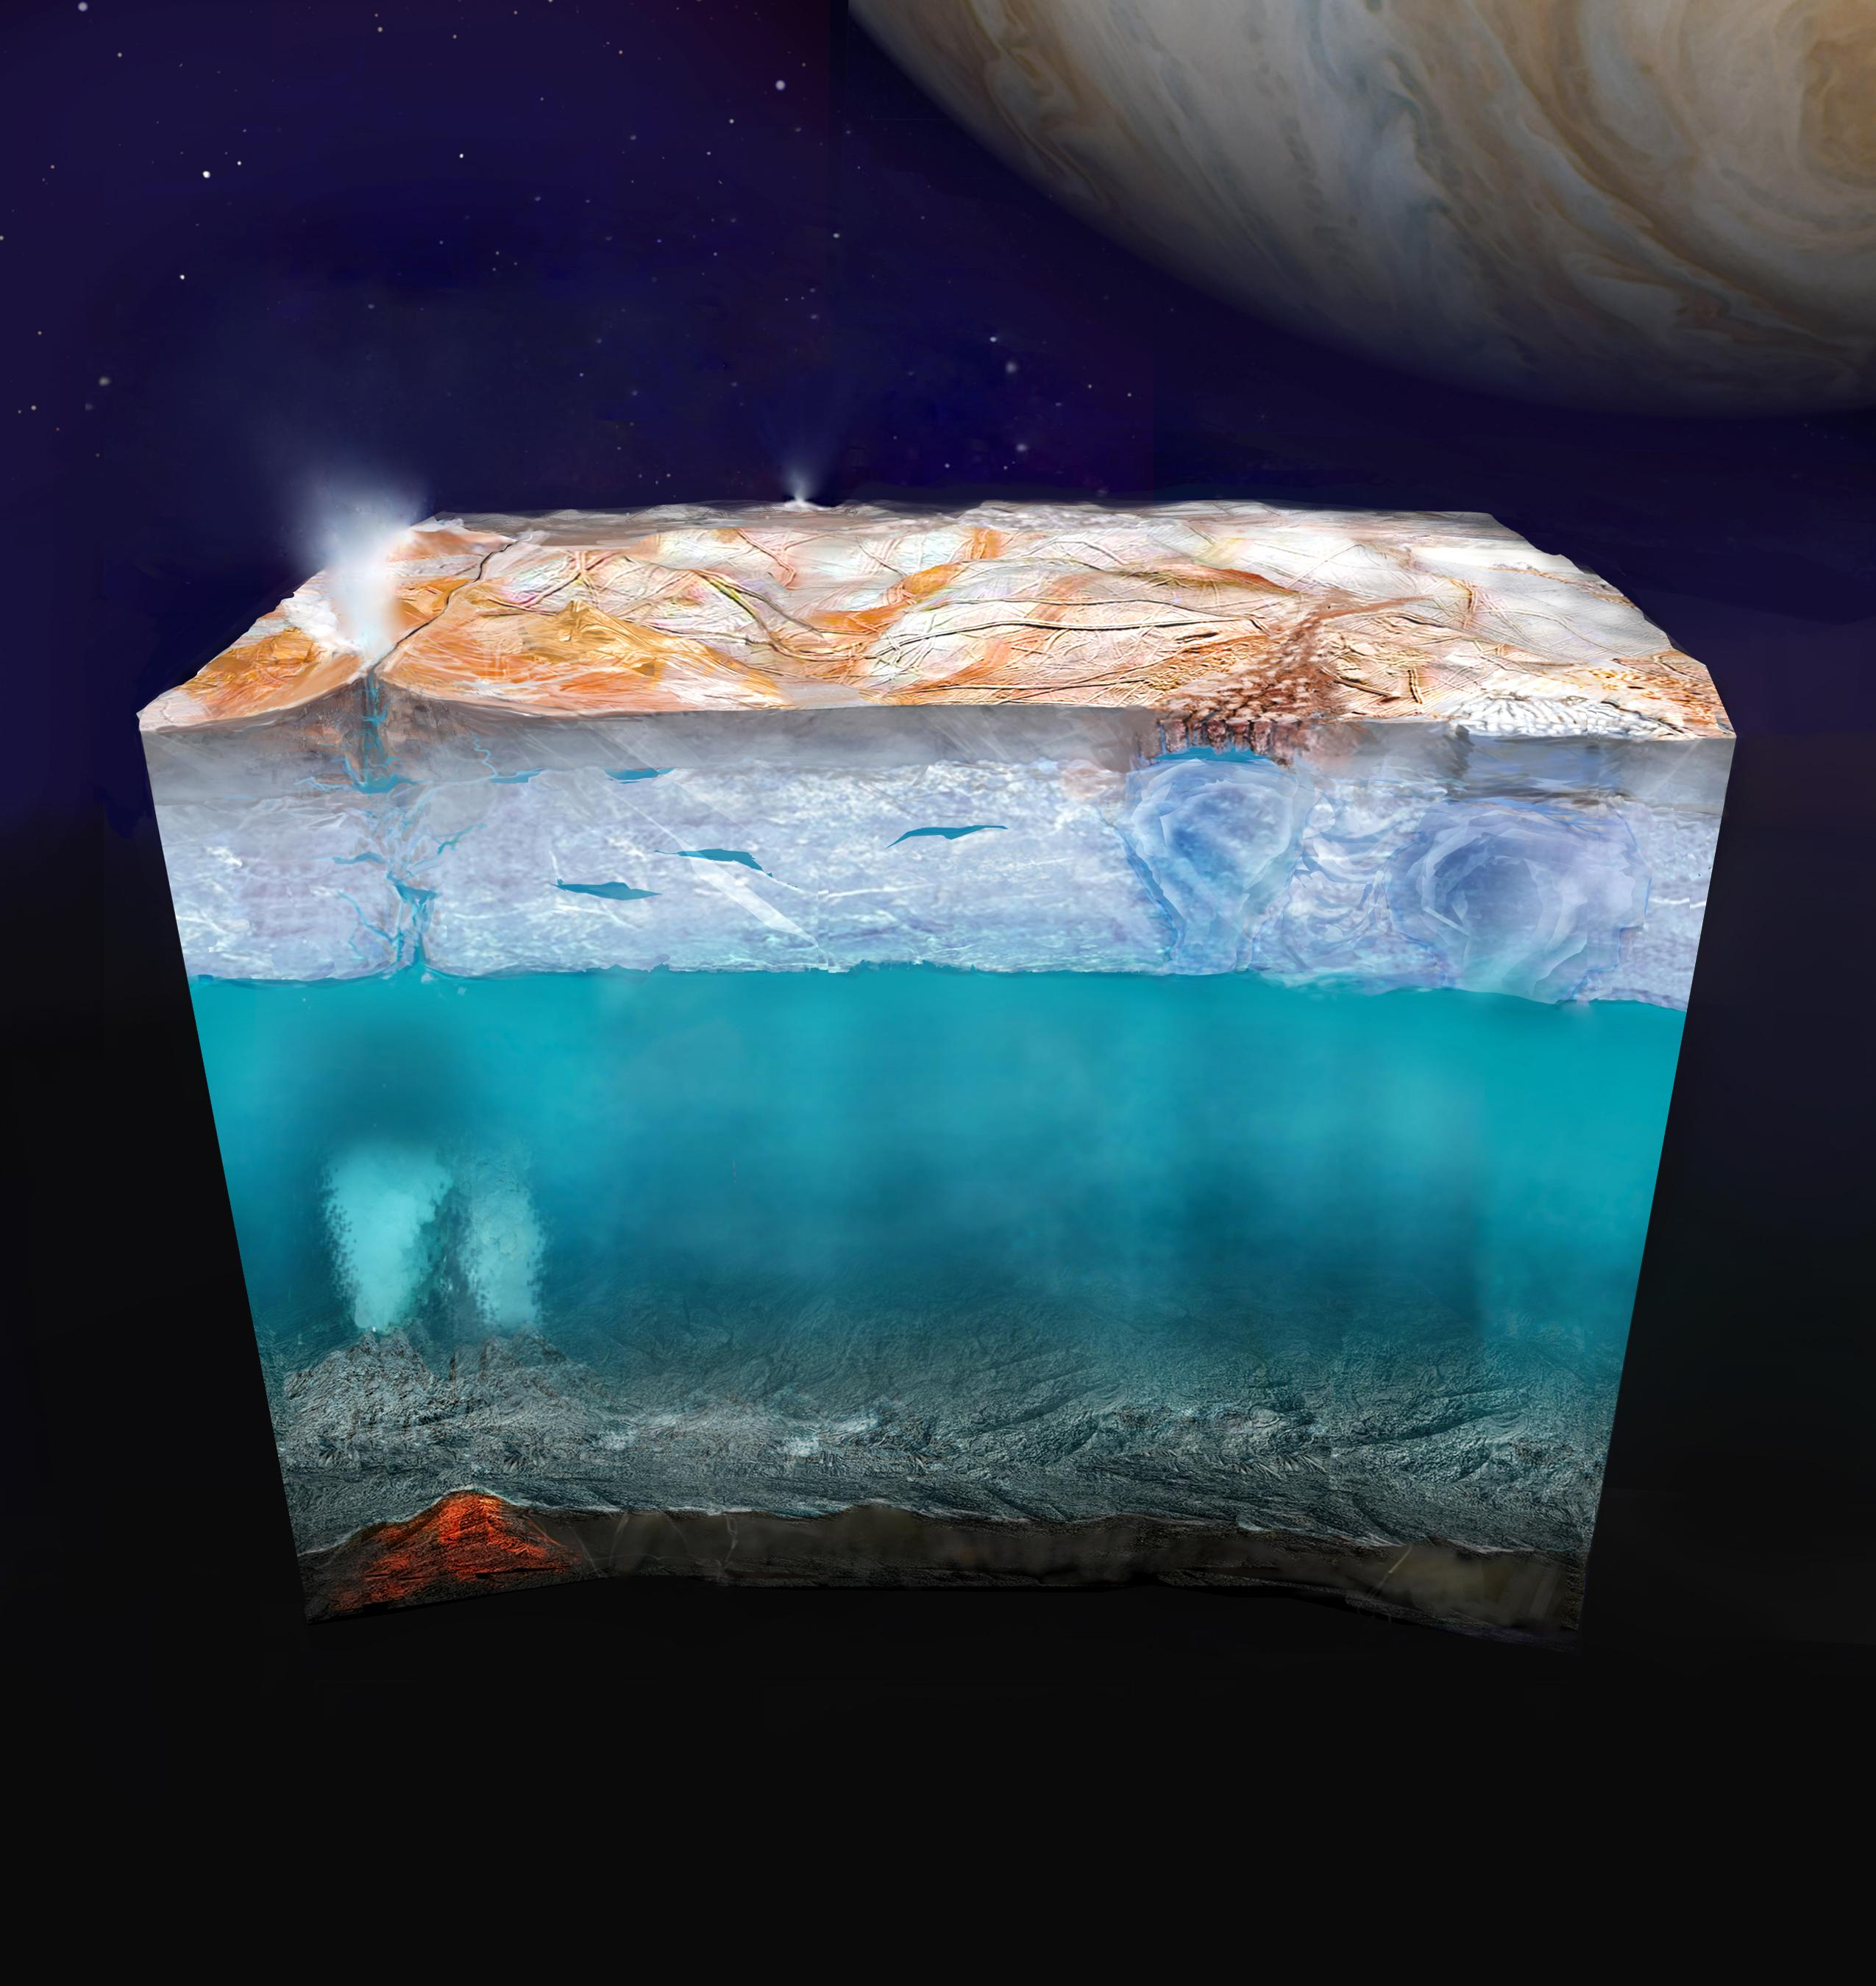
\includegraphics[width=0.25\textwidth]{figures/europa_ice}}
		\quad
		\subfloat[][]{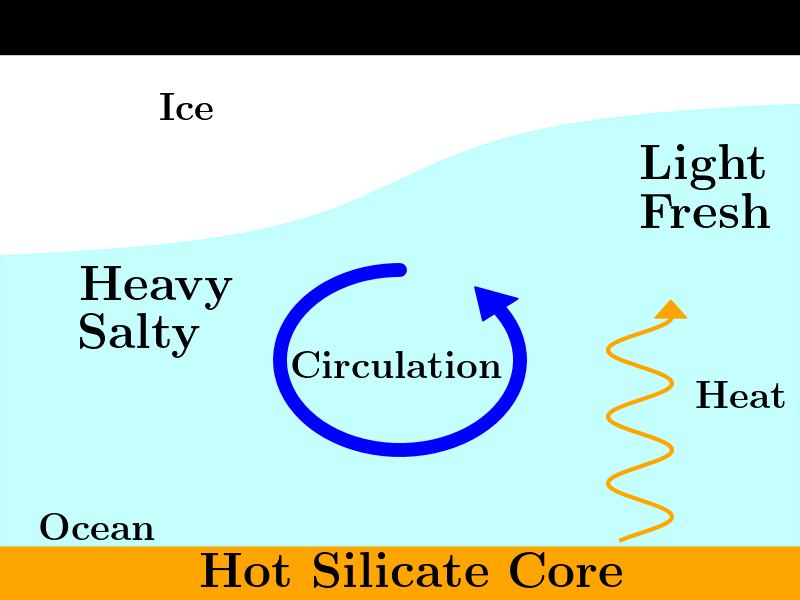
\includegraphics[width=0.35\textwidth]{figures/hc}}
	\subfloat[][]{\includegraphics[width=0.25\textwidth]{figures/conv}}
	\end{center}
	\caption{(a) Artist interpretation of subsurface ocean on Europa, not to scale (NASA/JPL-Caltech). (b) Possible mechanism for horizontal convection driven by heterogeneous melting. Adapted from \citep{wK22}. Snapshot of temperature from a simulation (by PI) of thermal bottom driven convection in a planetary core \citep{tO25}.}
	\label{f:pic}
\end{figure}

Two different mechanisms for convection will be considered.
Horizontal convection (HC) results from density heterogeneities on the icy surface. Heavy fluid sinks and light fluid flows in to replace it, as illustrated in figure \ref{f:pic}(b). This drives a circulation within the ocean. Bottom driven convection (BDC) is due to density differences between the fluid near the silicate core and the fluid at the icy surface. Lighter fluid near the core rises while heavier surface fluid sinks, once again setting up a circulation. 
%In plane layers, BDC is often referred to as Rayleigh-B\'enard convection. 
It is proposed that BDC is driven by radiogenic heating from the silicate core \citep{kS14,kS19,jK22}. A snapshot of a simulation of BDC in a planetary interior from the PI's dissertation is shown in figure \ref{f:pic}(c) \citep{tO25}. 
\textbf{In a rotating planet, heat fluxes due to BDC will vary with latitude \citep{kS14}. This indicates lateral variations in melt, which are expected to drive HC \citep{wK22}.}
The competition and interplay between these two mechanisms in spherical geometry, including the effects of rotation and salinity, is the purpose of the proposed project.


\section{Proposed project and methodology}

\textbf{In this project I propose to study the interaction between melt on the icy shell with the underlying convecting ocean via numerical simulations of a coupled ice-ocean system.} This will be the first study to consider thermal and saline convection in a full spherical geometry.
I will focus on the heat flux through the icy shell, and use these results to make predictions about temperature distributions and melt on the icy moons. These predictions will directly serve the upcoming the \textit{Europa Clipper} and \textit{JUICE} missions.

There are two major technical challenges associated with this study. The first is that it is not possible to perform fluid simulations in the actual parameter regimes of the icy moons. The second is generating a consistent model for heat fluxes into the ice and the resulting melt and release of fresh water.
In the following two sections, I outline my approach to handle these difficulties.
\subsection{Key nondimensional parameters}
\begin{figure}
	\begin{center}
		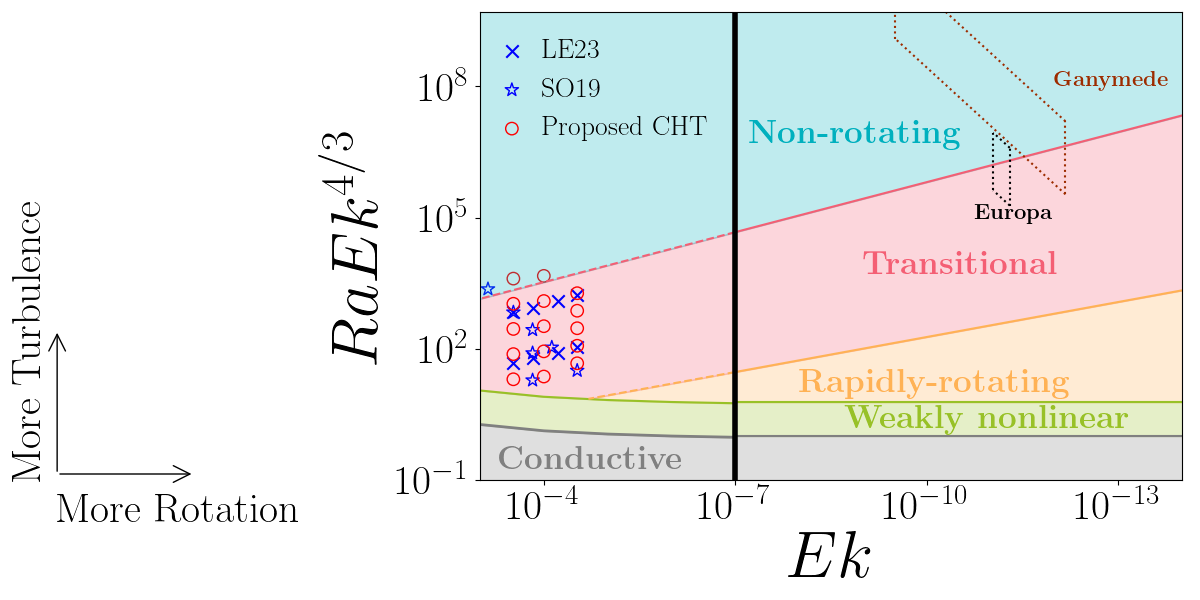
\includegraphics[width=0.7\textwidth]{figures/reg_diagram}
		\phantom{Lorem ipsum dolor sit amet}
	\end{center}
	\caption{Regime diagram for rotating convection, adapted from \citep{dL23,tG16}. Dashed lines - extrapolations of asymptotic predictions into the DNS region. Crosses and stars - parameter space from Lemasquerier et al. 2023\citep{dL23} and Soderlund 2019\citep{kS19} respectively. Regions enclosed by dotted lines represent approximate parameter space for Europa and Ganymede \citep{dL23,kS19}. Red markers indicate proposed simulations for conjugate heat transfer (CHT) study.
	}
	\label{f:reg_d}
\end{figure}
In convection studies, we solve dynamical equations governing the conservation of energy, momentum, and salinity. However, there is a large disparity between the scales relevant to planetary bodies and the scales that can be simulated. 
Usually this issue is formalized in terms of nondimensional numbers that represent the ratios of different physical effects in the system. %Alterntively, we can think of these quantities as ratios of different forcing terms in the governing equations. 
%In a geophysical and astrophysical context, there are two non-dimensional numbers of particular importance: the Rayleigh and Ekman numbers. 
The Rayleigh number $Ra$ describes the ratio of buoyancy to diffusivity. In planetary interiors, $Ra$ is very large, generally indicating vigorous convective turbulence.
The Ekman number $Ek$ is the ratio of viscous diffusion to Coriolis effects. Values for $Ek$ tend to be very small, indicating that rotation plays an important role.
For salty oceans, a buoyancy ratio $\Gamma$ quantifies the relative effects of temperature and salinity on density.
%Two other quantities of importance are the Nusselt number, $Nu$, and Prandtl number, $Pr$. 
%They are the ratio of total heat transfer to conductive heat transfer and the ratio of momentum to thermal diffusivity respectively \citep{kS19}. 
Explicitly, these parameters are
\[Ra = \frac{g\alpha\Delta T D^{3}}{\nu\kappa_{T}},\quad Ek = \frac{\nu}{\Omega D^{2}},\quad \Gamma = \frac{\alpha\Delta T}{\beta \Delta S}\]% \quad Nu = \frac{hD}{k_{O}} \quad Pr= \frac{\nu}{\kappa_{T}},\]
where $g$ is the surface gravitational acceleration, $\alpha$ and $\beta$ are the coefficient of thermal and saline expansion respectively, $D$ is the ocean thickness, $\nu$ and $\kappa_T$ are the diffusivities of momentum and temperature respectively, and $\Omega$ is the planetary rotation rate.
%, $h$ is the total heat transfer, and $k_O$ is the thermal conductivity of the ocean. 
$\Delta T$ is the temperature difference between the ocean surface and floor. $\Delta S$ is the average ocean salinity. 

The aspect ratio is the ratio of ocean thickness to planet radius. Estimations for the icy moons place this value around $0.1$\citep{sV18}, which is much smaller than the convection zone of the sun or the Earth's liquid core. As a result, the values of $Ek$ that can be simulated for the icy moons are much larger than those for the liquid core.
The aspect ratio will be fixed at $0.1$, which is identical to previous studies \citep{dL23,kS19}.

The Biot number, \textit{Bi}, is the ratio of conductive resistance to convective heat flow \citep{jL24}. A large value of $Bi$, relevant to icy moons, indicates that convective processes are important to determine the ice-ocean temperature response.
In our simulations $Bi$ is an output value, but we can control it by varying $D_{i}$, the thickness of the ice layer. 

%A compositional Rayleigh number $Ra_{S}$ can be defined by replacing $\alpha, \Delta T,\text{ and, }\kappa_{T}$ with the associated quantities for salinity.

To take Europa as an example, predicted values of $Ra$,  $Ek$, and $Bi$ are $O\lb 10^{20}\rb $, $O\lb 10^{-12}\rb $, and $O\lb 10^{6}\rb $ respectively \citep{dL23}. $\Gamma$ is poorly constrained but estimates suggest it is much less than unity \citep{yA21}. In the context of icy moons, numerical simulations have only reached values of $Ra \le 10^{9}$ and $Ek \ge 10^{-6}$ \citep{dL23}. 
%In studies of different planetary bodies, more aggressive simulations have been performed (eg. figure \ref{f:pic}(b), references \citep{tO25}), however all fall significantly short of reaching realistic values. For icy moons, it is particularly difficult to reach small values of $Ek$ because the ocean depth is much smaller than the planetary radius. 
\textbf{The procedure is to establish scaling laws with the nondimensional parameters by simulating at moderate values, and then extrapolating to planetary values}. 
%$Bi$ can be varied by simulating at different values of $D_{i}$. 
Prior work \citep{yA21} considered thermal and saline convection, but only for single values of $Ra$ and $Ek$, which prohibits extrapolation to extreme values.

Choosing which parameter space to investigate is difficult. 
Extreme parameter values (large $Ra$ and small $Ek$) is always desirable, but necessitates large numerical resolutions.  Therefore, a balance needs to be struck between parameter values and computational cost. 
A further complication, specific to rotating convection, is that flow behaviors are known to occupy a variety of regimes depending on values of both $Ra$ and $Ek$\citep{tG16}.
Figure \ref{f:reg_d} displays a cross-section of $Ek,Ra$ parameter space, and recognized convective regimes \citep{tG16}. The ordinate is $RaEk^{4/3},$ which determines the boundary between conduction and convection\citep{sC61}.

As $Ek\rightarrow 0$, rotational effects dominate the system and suppress radial motion. The ``conductive,'' ``weakly non-linear,'' and ``rapidly rotating'' regimes\citep{tG16,kJ12} are all characterized by axially stretched flows conforming to the Taylor-Proudman (TP) theorem at leading order. TP dictates that rapidly-rotating flows remain invariant along the axis of rotation \citep{gB53}.
%As $Ra$ is increased, convection sets in as axially stretched flows conforming to the Taylor-Proudman theorem \citep{gB53}, which dictates that rapidly-rotating flows remain invariant along the axis of rotation. Such dynamics are known as geostrophic.
%Geostrophic flows are laminar over a small range of $Ra,$ but quickly become turbulent. Geostrophy holds over large time and length scales, but on small scales low order fluctuations make the dynamics highly non-linear.
%This regime is often referred to as ``rapidly rotating'' or ``geostrophic turbulence'' \citep{kJ12}.

Further increase of $Ra$ yields the ``transitional" regime, where the TP constraint is significantly relaxed, but flows are still rotationally influenced.
Eventually, flows become turbulent enough that rotation's role is minimal. This regime is labeled ``non-rotating.''
Although significant uncertainty exists, it is believed that the icy-moons lie in the transitional and non-rotating regimes\citep{dL23,tG16}.

%Forward models in this regime\citep{kS19, dL23}, have investigated only the liquid ocean and do not consider the effects of salinity. 
The parameter space that I will explore is provided in table \ref{t:param}. Overlap with previous studies \citep{dL23,kS19} is intended, as it will allow me to compare my findings with these ``purely thermal" results. This will better elucidate the added effects of saline convection.
%I will explore similar parameters to the regimes studied in references \citep{dL23,kS19}. This will allow me to best compare these ``purely thermal'' results to my findings, which will better elucidate the new effects of saline convection. 
I will sweep across an order of magnitude in $\Gamma$ to establish a scaling relationship with the buoyancy ratio. 
%A complete list of the proposed simulations is given in table \ref{t:param}. 
\subsection{A dynamically coupled ice-ocean model}

Horizontal convection is driven by salinity variations at the outer boundary of the liquid domain. In order to investigate this mechanism, it is necessary to couple the heat fluxes into the ice with melt into the ocean. 
Convective studies that do not consider salinity have generally only investigated the ocean \citep{kS19,dL23} and not the ice. The general approach is to fix the temperature of the bounding surface (ice shell), however this implies uniform melt.
\textbf{I propose to use a simulation configuration in which the ice is included in the solution domain so that heat is able to conduct from the ocean into the ice.} 
A boundary condition for temperature is placed on the moon surface, and the temperature of the ocean-ice interface is allowed to vary. The interfacial temperature can be used to determine the salinity at the ocean surface \citep{wK22}.
\textbf{This approach has never been used in a full spherical geometry.}\\

I will supplement these global simulations with a suite of ``local" simulations in a cartesian plane layer. By reducing the effective volume of the domain, Local models allow for more extreme values of $Ra$ and $Ek$, which helps to validate scaling laws based on the global results. Although local models miss some physics captured by global models, they share many fundamental processes and allow for the investigation of more turbulent flows.


\begin{table}
\begin{center}
\begin{tabular}{|c|c|c|c|c|c|c|}
\hline
Model&$Ra$&$Ek$&$D_{i}/D$& $\Gamma$ &\# Simulations & cpu$\times$hour\\
		\hline
G&$\lb 5 \times 10^{6} - 2 \times 10^{8} \rb $ & $3 \times 10^{-4} $ & $0.5,0.1$&0.5,0.05&20&$1.7 \times 10^{6}$\\
  	\hline
G&$\lb 5 \times 10^{6} - 1 \times 10^{9} \rb $ & $1 \times 10^{-4} $ & $0.5,0.1$&0.5,0.05&20&$1.7\times 10^{6}$\\
  	\hline
G&$\lb 5\times 10^{7}, 2 \times 10^{9} \rb $ & $3 \times 10^{-5} $ & $0.5,0.1$&0.5,0.05&8&$2.5\times 10^6$\\
		\hline
%Shell & $10^5$& $\infty$&$10^4-10^5$& 5& $2\times 10^{6}$\\
%		\hline
%Shell & $10^5$& $10^{-4}$&$10^4-10^5$& 5& $2\times 10^{6}$\\
%		\hline
%Plane &$5\times10^{5}-2\times10^{6}$ & $3\times10^{-4}$&$12.5Ra$ &5 &$2.5\times 10^{5}$  \\
%		\hline
%Plane &$10^{6}-10^{7}$ & $10^{-4}$&$12.5Ra$& 5 & $5\times 10^{5}$\\
%		\hline
%Plane &$10^{7}-5\times 10^{7}$ & $3\times10^{-5}$&$12.5Ra$ & 5& $10^{6}$ \\
		\hline
Totals & && & &48&$4.9 \times 10^6$ \\
		\hline
\end{tabular}
\end{center}
\caption{Proposed parameter space. G refers to a global model in a full spherical shell. L refers to a local model in a cartesian plane. The third column presents the ratio of ice to ocean thickness, which can be modified to change $Bi$. Computing costs are estimate values based off of existing studies \citep{dL23,rM19} and personal experience with relevant codes.}
\label{t:param}
\end{table}


\subsection{Proposed simulations and computing requirements}
I propose a suite of 48 simulations to investigate ice-ocean coupling in the icy moons. The specific parameter values are given in table \ref{t:param}, as well as the estimated computing cost.  The existing hydrodynamics code \texttt{Nek5000} \citep{nek5000} will be used to perform the simulations, and can be configured to handle thermal-saline convection as well as the solid icy exterior.
In previous work \citep{tO25}, I have used \texttt{Nek5000} to investigate core mantle interactions in the Earth's liquid core and have extensive experience with running and modifying the code. Table \ref{t:param} provides estimate computing times based on previous rotating convection studies in icy moons \citep{dL23} and my experience with \texttt{Nek5000}.
 I will apply for computing time through ACCESS and the Texas Advanced Computing Center, which both provide access to high performance computing resources and have supported me in the past. The proposed host institution, UC San Diego, can also provide computing time.
 \subsection{Timeline}
 Completion of this project will require three years. The proposed model has yet to be built and significant effort will be required to construct and test it.\\
 Years 1-2 - \textit{Local model and code development}\\
 The global and local models need to be built within the \texttt{Nek5000} framework. Additionally, tools need to be built to analyze results. It is most efficient to perform analysis as the simulation is performed, which means it is best practice to develop analysis tools before simulations are started. Once these tools are built, I will run the local model.
 The local model will require less computational resources and can be used to gauge the feasibility of the proposed parameter regime for the spherical model. At least one paper is expected from these results.\\
 Year 2 - \textit{Global model}\\
  Simulations for the global model will begin once feasibility of the proposed parameters is determined. A study comparing local and global results will be performed. At minimum of two papers are expected from global model results. \\
 Year 3 -  \textit{Observational significance}\\ I will focus on developing predictions that can be tested by upcoming missions and observations of the surfaces of icy moons and exoplanets. A minimum of one paper will result from this work.

\section{Intellectual Merit}
The presence of an ocean indicates that a planet may be habitable\citep{tB24}. The icy moons of Jupiter and Saturn are known to contain subsurface ocean and many terrestrial exoplanets are expected to contain oceans beneath an icy layer as well\citep{lQ20}. The dynamics of these oceans are not well understood. As a result, whether and how these dynamics leave a signature on the ice above is unknown. It will be useful for current and future missions to have models that dynamically link the ice to the subsurface oceans.

\subsection{The Moons of Jupiter and Saturn}
The primary objective of NASA's \textit{Europa Clipper} (EC)\cite{pC14_EC} and ESA's \textit{JUICE} \citep{oG13} missions is to investigate Europa, Ganymede, and Callisto, three Jovian satellites believed to be ocean worlds. Each is expected to contain salty, liquid oceans underneath thin icy shells \citep{rP99,fN16}, and both EC and \textit{JUICE} aim to determine whether these bodies contain necessary conditions for life \citep{tB24}. 

The dynamics of these oceans are poorly understood, and neither mission will be able to make direct observations of the oceans, however multiple observations are planned that will hint at the ocean dynamics. For example, EC will use radar altimetry to determine surface topography and a magnetometer to constrain salinity profiles with depth \citep{jR23}.  
A deeper understanding of the interaction between the convection and icy surface is necessary, and is outlined as one of the key future issues in the recent review of icy moon oceanography \citep{kS24}.


The proposed study will investigate the thermal response of the icy shell to the underlying convection, and the ocean's response to the melting and freezing shell. 
%\textbf{When data from EC and \textit{JUICE} becomes available, these results will provide insight into the interior of the Jovian ocean worlds.}
\textbf{These results will provide insight into the interior of the Jovian ocean worlds, which will be crucial to interpret the upcoming data from EC and \textit{JUICE}.}
%\subsection{Beyond the Jovian system}

This project applies to other planetary bodies as well. The Saturnian moon Enceladus likely contains a sub-surface ocean and has a similar geometry to Europa \citep{kS24}. There is significant uncertainty whether Triton \citep{jK22} and Pluto \citep{kS24} are ocean worlds and the results of this study will be useful to further constrain the properties of these bodies. 

\subsection{Beyond the Solar System}
Significantly less is known about exoplanets, although it has been predicted that many known exoplanets contain subsurface oceans\citep{lQ20}. Near-term missions will be unable to acquire detailed information about the surface, however surface temperatures and compositions have been reported for tens of exoplanets\citep{nM19}. The results of this project may be able to use the results to identify an ocean. 
Little is known about the interior dynamics of exoplanets. The results from this proposal can be used to make predictions about surface heat flux and surface ice thickness given a particular set of nondimensional parameters. In the future, these predictions could be coupled with observations to determine the convective regimes of exoplanet oceans. This has implications for determining whether these planets can host a planetary dynamo\citep{pD11}.
Furthermore, the proposed work can be generalized beyond salty oceans. The governing equations are, agnostic to the actual fluid and buoyancy sources. Fluid parameters are identified by only the values of $Pr$ and $Sc$, so that we should be able to draw conclusions about liquid layers of any type. This includes liquid metal layers similar to the core of the Earth. This may be relevant to exoplanets too warm to contain an icy sheet.

Lastly, the studied convective processes have implications for induced magnetic fields and planetary dynamos. Our results will be useful in investigating the magnetic properties of planetary bodies in the Solar System and beyond.

\section{Proposed institution- UC San Diego}
%Dr. Young and Dr. Siegelman are faculty at Scripps Institution for Oceanography (SIO) at UC San Diego. 
I propose to work with Dr. Lia Siegelman and Dr. William Young, who are physical oceanographers at Scripps Institution for Oceanography (SIO) at UC San Diego. 
They have recently investigated astrophysical fluid mechanics in the context of Jovian polar dynamics and the formation of the polar vortex crystals\cite{lS22,lS22b,lS24}, and are interested in icy moon ocean dynamics and the proposed project involved input from both.

\subsection{An interdisciplinary approach to extraterrestrial oceans}
My research has been primarily focused on geophysical turbulence in the context of the Earth's liquid core. Although the fluid dynamics of the liquid core and terrestrial oceans share many similarities, fundamental differences exist in both the physical problem and the scientific approaches. Terrestrial oceans are, relative to their lateral extent, very thin layers, whereas the liquid core is relatively thick. This leads to significantly different mathematical and numerical approaches when attempting to solve the dynamics.
The oceans of the icy moons almost certainly fall in an intermediate regime between the liquid core and the Earth's oceans, and therefore insight from both fields is required of any investigation. The literature on compositional convection is far richer in the oceanographic context because of the large role that salinity plays in the oceans, and I would benefit greatly from working with both Dr. Siegelman and Dr. Young since saline horizontal convection is a major focus of this project. 
Ice-ocean interactions are also relevant, and Dr. Siegelman has recently been involved in multiple studies (\textit{in prep}) on sea-ice interactions. 
%More broadly, access to the facilities and faculty at SIO would be invaluable to me with respect to \textcolor{red}{ammending knowledge gaps in oceanography}. 
\textbf{Study of the oceans of the icy moons is at the intersection of physical oceanography and planetary-scale, deep convection. My background in core convection partners well with the oceanographic expertise of Dr. Siegelman and Dr. Young.}

\subsection{Collaboration with icy moon surface experts}
The Department of Astronomy and Astrophysics is a new department (est. 2023) at UC San Diego, and is the home department of Dr. Samantha Trumbo. Dr. Trumbo is a planetary scientist and expert on Europa surface processes. 
A primary goal of the proposed project is to relate theoretical predictions of ocean convection to surface processes. The opportunity to collaborate with Dr. Trumbo would improve our understanding of the capabilities of the \textit{Europa Clipper} mission and allow us to better identify surface indicators of identified ocean processes.

%They connect elementary through high school students with researchers to learn about the research at SIO.
\section{Broader Impacts}

\subsection{Long term goals}
This fellowship would broaden my scientific expertise. Through graduate school,
the focus of my research has been convection in planetary interiors similar to the Earth's core, but I would like to increase my research perspectives to include other planetary bodies and terrestrial oceans. Most of my research has been purely numerical, with highly idealized models that are poorly constrained by data. This is due largely to the lack of observational results for planetary interiors. In contrast, the oceanography community often works with parameterized models such as the \texttt{MITgcm}\citep{jM97} that can, in principle, reach much more extreme parameter regimes. The icy moons are a crossroads between planetary convection and oceanography and present an exciting natural laboratory for studying rotating convection where new data is upcoming. I would personally benefit from this fellowship because it would expose me to the oceanographic approach to convection problems, and would improve my outlooks when applying for research positions in the planetary sciences. More broadly, I think that the planetary interiors community and the oceanography community would benefit from more collaboration. 


\subsection{Public outreach at SIO}
The SCOPE program at SIO coordinates outreach opportunities between San Diego students and researchers. 
I want to participate in this program by performing rotating tank demonstrations, which are fun, simple experiments that engage students in planetary science.
%
\section{Education Plan}
I think that it is important to create spaces where students can share ideas without the pressure of expectations from their advisors and other faculty.
CU-Prime\citep{cup} is a student-run mentorship program in my home department (University of Colorado Boulder, Department of Physics) that aims to create these spaces. 
I have worked with CU-Prime and propose to found and coordinate a similar program for undergraduate and graduate students at UC San Diego. In order to promote interdisciplinary science, I would start by including three departments: the Scripps Institution for Oceanography (SIO), the Department of Astronomy and Astrophysics (A\&A), and the Department of Physics (PHYS). 

I propose two aspects of this program. First, I will facilitate mentorship partnerships between undergraduate and graduate students. Second, I will coordinate a bi-weekly talk series in which graduate students present their research to a general undergraduate audience. 

\subsection{Graduate mentorship partnerships}
At the beginning of each academic year I will recruit second year and older graduate students to serve as volunteer mentors for small (4-6) person pods of undergraduates and first year graduate students (mentees). Pods will be scheduled to meet twice each semester to discuss classwork, getting involved in research, and advice for succeeding in their programs. 
Pods will be formed such that each group of students will represent a variety of scientific interests from SIO, A\&A, and PHYS. 
This partnership will provide leadership opportunities for the mentors, and will increase access to research and science networks for the mentees.
\subsection{Talk series}
I will also coordinate a talk series for graduate students to present their research. The intended audience are undergraduates in physics, planetary science, and geosciences, and so a lot of effort will go into working with the speaker to make sure that their talk is accessible, jargon-free, and well explained. Speakers will also be asked to discuss how they got involved in their current research and their path to graduate school. These talks will provide a low-stress environment for both the audience and the speaker.
The audience is provided with a window into what it actually means to be a scientific researcher, and how one might become one themselves, and the speaker is afforded a comfortable environment where they can practice presenting their research to a non-critical crowd.

As a graduate student I have prepared two talks under this format, and I have found them to be very positive experiences. It was more difficult than I had thought to prepare these presentations, but I found that it helped me quite a bit when I was preparing conference talks later on. I was more confident, and I was better at communicating my findings, rather than overwhelming my audience with details. 

I expect the proposed program to require 5-8 hours per week. This estimate is based off of discussions with the current administrator of CU-Prime. 
\section{Significance beyond NASA's \textit{Europa Clipper}}
A major goal of this proposal is to determine the relationship between ocean convection and surface processes on icy moons, which includes Europa, Callisto, and Ganymede. In part, this is motivated by the upcoming \textit{Europa Clipper} mission, which will perform a variety of surface and magnetic measurement. I expect the results of this study will better inform our understanding of sub-surface dynamics as those results return. I do not, however, propose to use NASA resources or EC data in this project. The focus of this research is more broadly about icy moon dynamics than any particular observation. Furthermore, the scope of this project extends beyond EC. The \textit{JUICE} mission will also require extensive modeling to make sense of its results, and future observations and missions will benefit from the proposed work, regardless of the source.

\begin{spacing}{0.4}
%\begin{multicols}{2}
%\bibliography{References,journal_abbreviations}%jfm-bib,References}

\printbibliography

%\end{multicols}
\end{spacing}
\end{document}
